\section{Software}
\begin{frame}[t]{Software}
    \only<+->{Can we make this \stress{easy} for everyone? }
    
    \only<+->{
        \vspace{-0.4cm}
        {\raisebox{0.3cm}{\scalebox{1.3}{\color[gray]{0.4}\texttt{https://github.com/}}}\hspace{0.1cm}{
\includegraphics[height=1.6cm]{figures/software_logos/clusterking.pdf}}}
       
        \vspace{-0.25cm}\hspace{4.2cm}{\ckBlue\underline{Cluster}ing \color{black}of \ckRed\underline{Kin}ematic \ckYellow \underline Graphs}
        
        \vspace{0.5cm}
        
        Our project is \stress{openly} developed on
        \vcenteredinclude{
\includegraphics[height=2ex]{figures/software_logos/octocat.pdf}\hspace{-0.05cm}
           
\includegraphics[height=2ex]{figures/software_logos/github.pdf}} \\\srem{(in fact even this presentation is there)}\\
        %{\color{purple}\url{https://github.com/clusterking}}
        \vspace{-0.9cm}
    }
    
    \only<+->{
        \vspace{1cm}
        Implemented in \vcenteredinclude{
\includegraphics[height=3ex]{figures/software_logos/python.pdf}} using
        \begin{columns}
            \column{0.5\linewidth}
            \begin{itemize}
                \item \vcenteredinclude{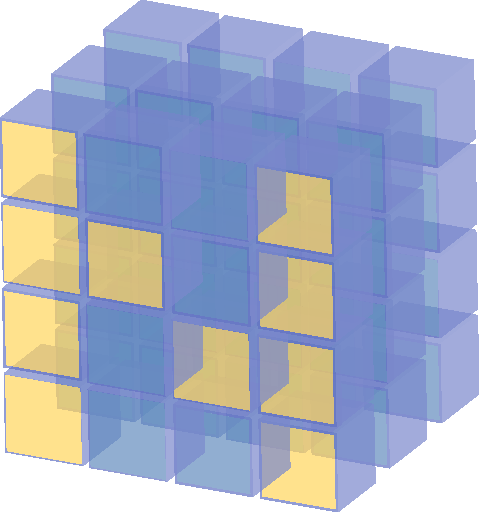
\includegraphics[height=4ex]{figures/software_logos/numpy_noname.pdf}} \texttt{numpy} {\footnotesize(fast numerics)}
                \item \vcenteredinclude{
\includegraphics[height=4ex]{figures/software_logos/pandas_noname.pdf}} \texttt{pandas} {\footnotesize(dataframes)}
                \item \vcenteredinclude{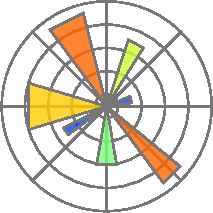
\includegraphics[height=4ex]{figures/software_logos/matplotlib.pdf}} \texttt{matplotlib} {\footnotesize(beautiful plots)}
                \item \vcenteredinclude{
\includegraphics[height=4ex]{figures/software_logos/sklearn_small.pdf}} \texttt{scikit-learn} {\footnotesize(clustering)}
                \item \vcenteredinclude{
\includegraphics[height=4ex]{figures/software_logos/scipy.pdf}} \texttt{scipy} {\footnotesize(integration and clustering)}
                %\item 
            \end{itemize}
            \column{0.5\linewidth}
            \begin{itemize}
                \item \vcenteredinclude{
\includegraphics[height=4ex]{figures/software_logos/jupyter.pdf}} \texttt{jupyter} {\footnotesize(interactive notebooks)}
                \item \vcenteredinclude{
\includegraphics[height=4ex]{figures/software_logos/wcxf.pdf}} \texttt{wcxf} {\footnotesize(Wilson coefficients)}
                \item \vcenteredinclude{
\includegraphics[height=4ex]{figures/software_logos/wilson.pdf}} \texttt{Wilson} {\footnotesize(Wilson coeff. running)}
                \item 
                \vcenteredinclude{
\includegraphics[height=3.5ex]{figures/software_logos/sqla.png}} {\footnotesize (Output format)}
                \item \vcenteredinclude{
\includegraphics[height=4ex]{figures/software_logos/flavio.pdf}} \texttt{Flavio} {\footnotesize(Observables)}
            \end{itemize}
         \end{columns}
     }
     \only<+->{
         \vspace{0.1cm}
         \begin{center}
             Installation: \ {\color{purple}\texttt{pip3 install clusterking}}
        \end{center}
    }
\end{frame}

\begin{frame}{Software}
    \begin{itemize}
        \item \stress{Documentation} on \vcenteredinclude{
\includegraphics[height=2.5ex]{figures/software_logos/rtd_noname.pdf}} \texttt{Read the Docs}:\\[3ex]
        \begin{center}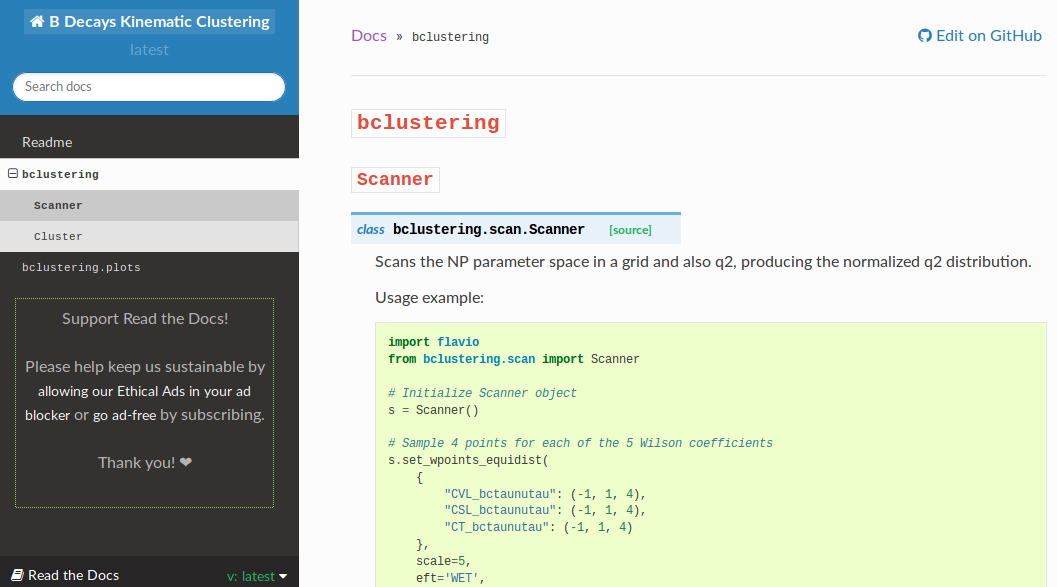
\includegraphics[width=0.8\linewidth]{figures/scrot/readthedocs.png}\end{center}
        \vspace{2ex}
        \item \stress{Interactive tutorials} using \vcenteredinclude{
\includegraphics[height=3.5ex]{figures/software_logos/jupyter.pdf}} \texttt{jupyter notebooks}\\
        Can also be run directly without installing anything (\vcenteredinclude{
\includegraphics[height=2.5ex]{figures/software_logos/binder_noname.pdf}} \texttt{binder})
        %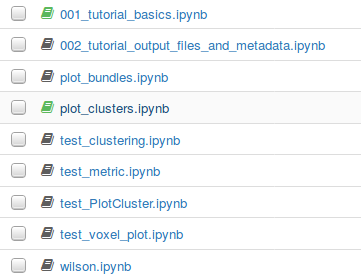
\includegraphics[width=3cm]{figures/scrot/jupyter.png}
    \end{itemize}
    
    \bigskip
    
\end{frame}

\begin{frame}{Software}
    \framesubtitle{Steps}
    \begin{enumerate}
        \item<+-> \stress{Scan}: Calculate distribution for sample points in parameter space\\
        {\footnotesize e.g. $\dd\Gamma/\dd q^2$ in Wilson space}
        \begin{itemize}
            \item Take arbitrary python functions (e.g. from \texttt{flavio})
            \item Parallel processing supported
        \end{itemize}
        \item<+-> \stress{Add uncertainties} (optional)\\
         %{\footnotesize(Poisson, flat relative errors, errors given by covariance matrix, max. correlated errors etc.)}
        \item<+-> \stress{Cluster}%: Take the binned distributions and cluster them\\
       % {\footnotesize Clustering class is subclassed to support any clustering algorithm}
        \item<+-> \stress{Benchmark points}%: Select one representative for each cluster
        \item<+-> \stress{Plot!}\\
        {\small Various plotting methods at your fingertips}
    \end{enumerate}
\end{frame}

\ifexamples
\begin{frame}[t, fragile]{Software}{Quick tutorial}
    Generate a sample of kinematic distributions using the \mintinline{python}{Scanner} class:\\
    {\footnotesize Here: $\dd\Gamma/\dd q^2$ for $\bdstaunu$}
    
    \only<1>{
        \inputminted[lastline=4]{python}{code/scan.py}
    }
    \only<2>{
        \inputminted[lastline=9]{python}{code/scan.py}
    }
    \only<3>{
        \inputminted[lastline=15]{python}{code/scan.py}
    }
    \only<4>{
        \inputminted[]{python}{code/scan.py}
    }

\end{frame}

\begin{frame}[fragile]{Software}{Quick tutorial}
    Now we cluster it: 
    
    \inputminted{python}{code/cluster.py}
    
    \begin{columns}
        \column{0.4\linewidth}
        And can directly plot it:
        
        \begin{changemargin}{0.32cm}{0cm}
        \begin{minted}[gobble=12]{python}
            d.plot_clusters_scatter([
                "CVL_bctaunutau",
                "CSL_bctaunutau",
                "CT_bctaunutau"   
            ])
        \end{minted}
        \end{changemargin}
        \column{0.6\linewidth}
        \centering
        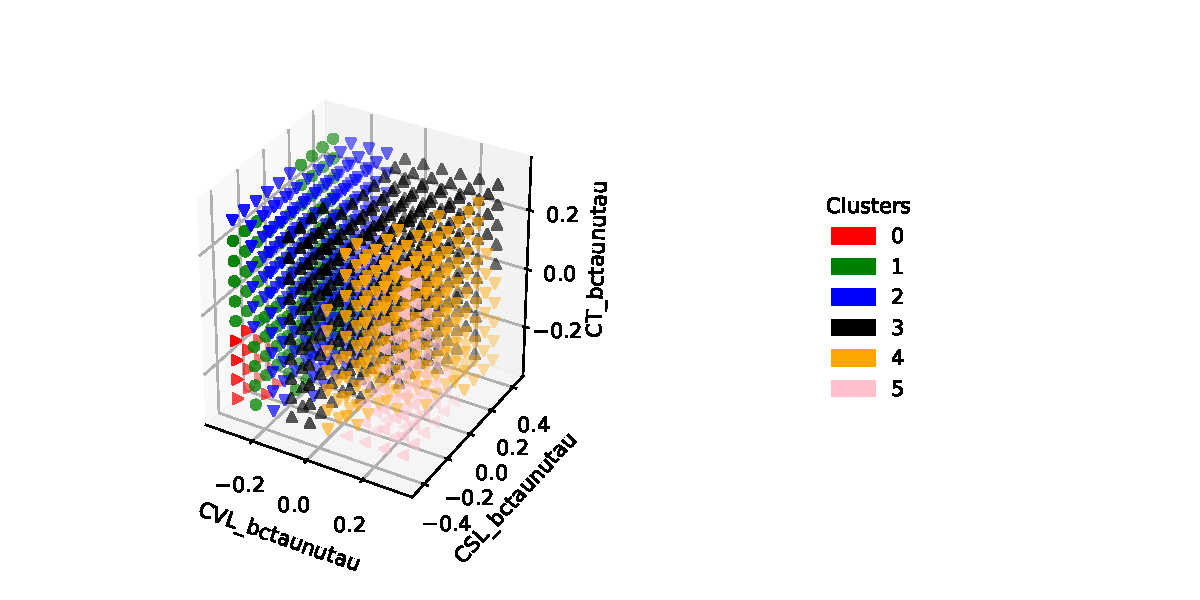
\includegraphics[width=5.5cm]{figures/plots/3d.pdf}
    \end{columns}
\end{frame}


\begin{frame}[fragile, t]{Software}{Quick tutorial}
\vspace{0.75cm}
\begin{minted}[gobble=4]{python}
    d.plot_clusters_scatter(['CVL_bctaunutau', 'CSL_bctaunutau'])
\end{minted}
\vspace{0.2cm}
\centering
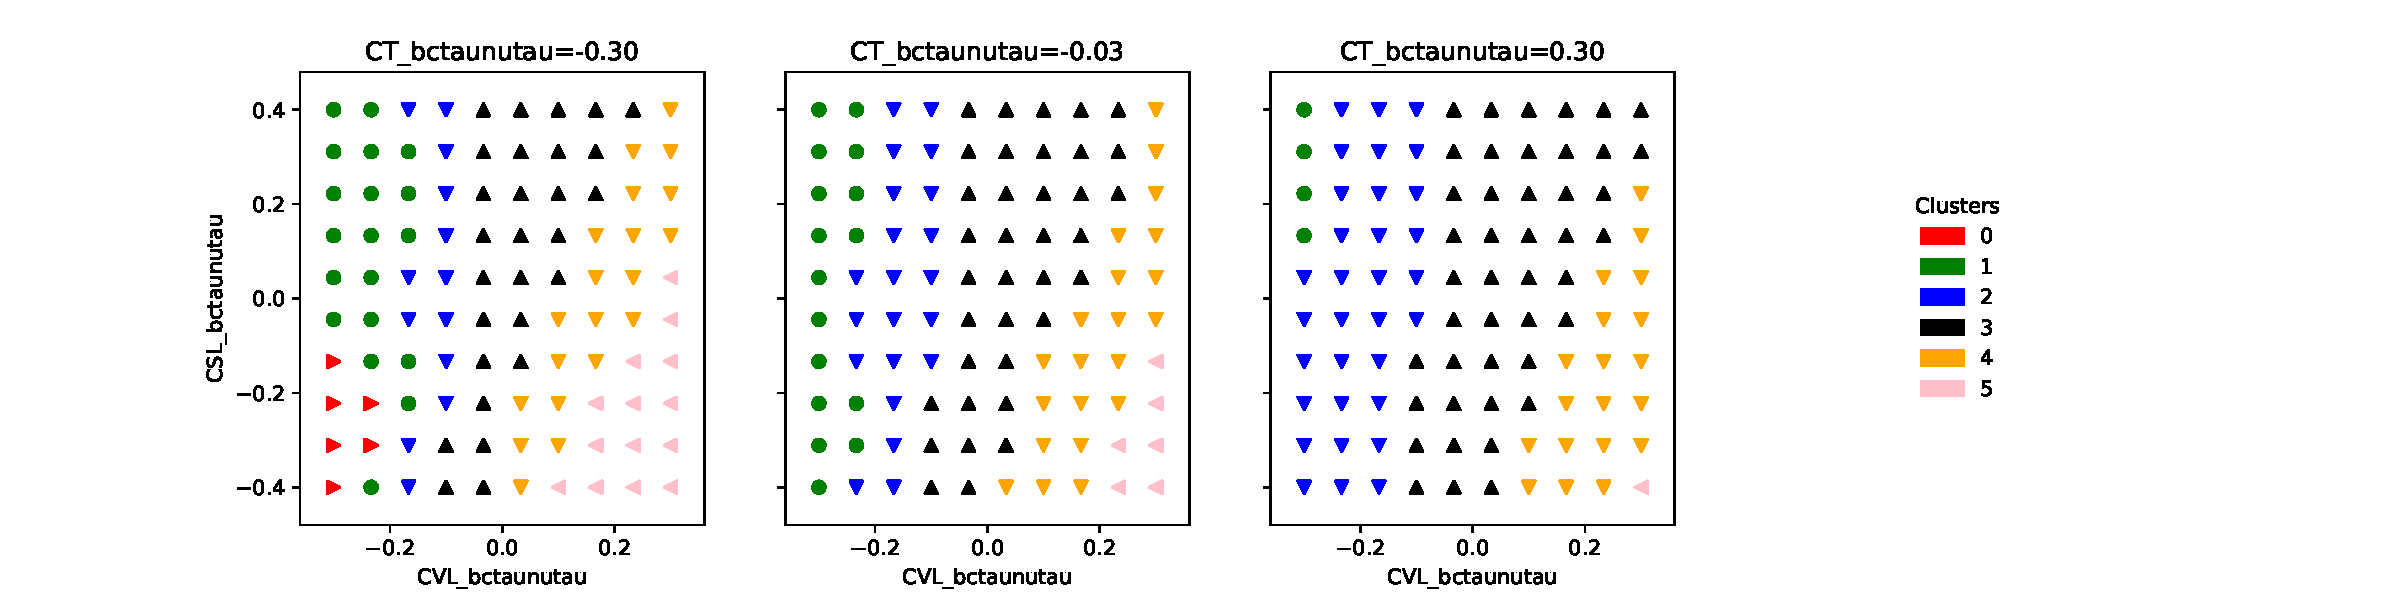
\includegraphics[width=10.5cm]{figures/plots/2dpoints.pdf}
\end{frame}

\begin{frame}[fragile, t]{Software}{Quick tutorial}
\vspace{0.75cm}
\begin{minted}[gobble=4]{python}
    d.plot_clusters_fill(['CVL_bctaunutau', 'CSL_bctaunutau'])
\end{minted}
\centering
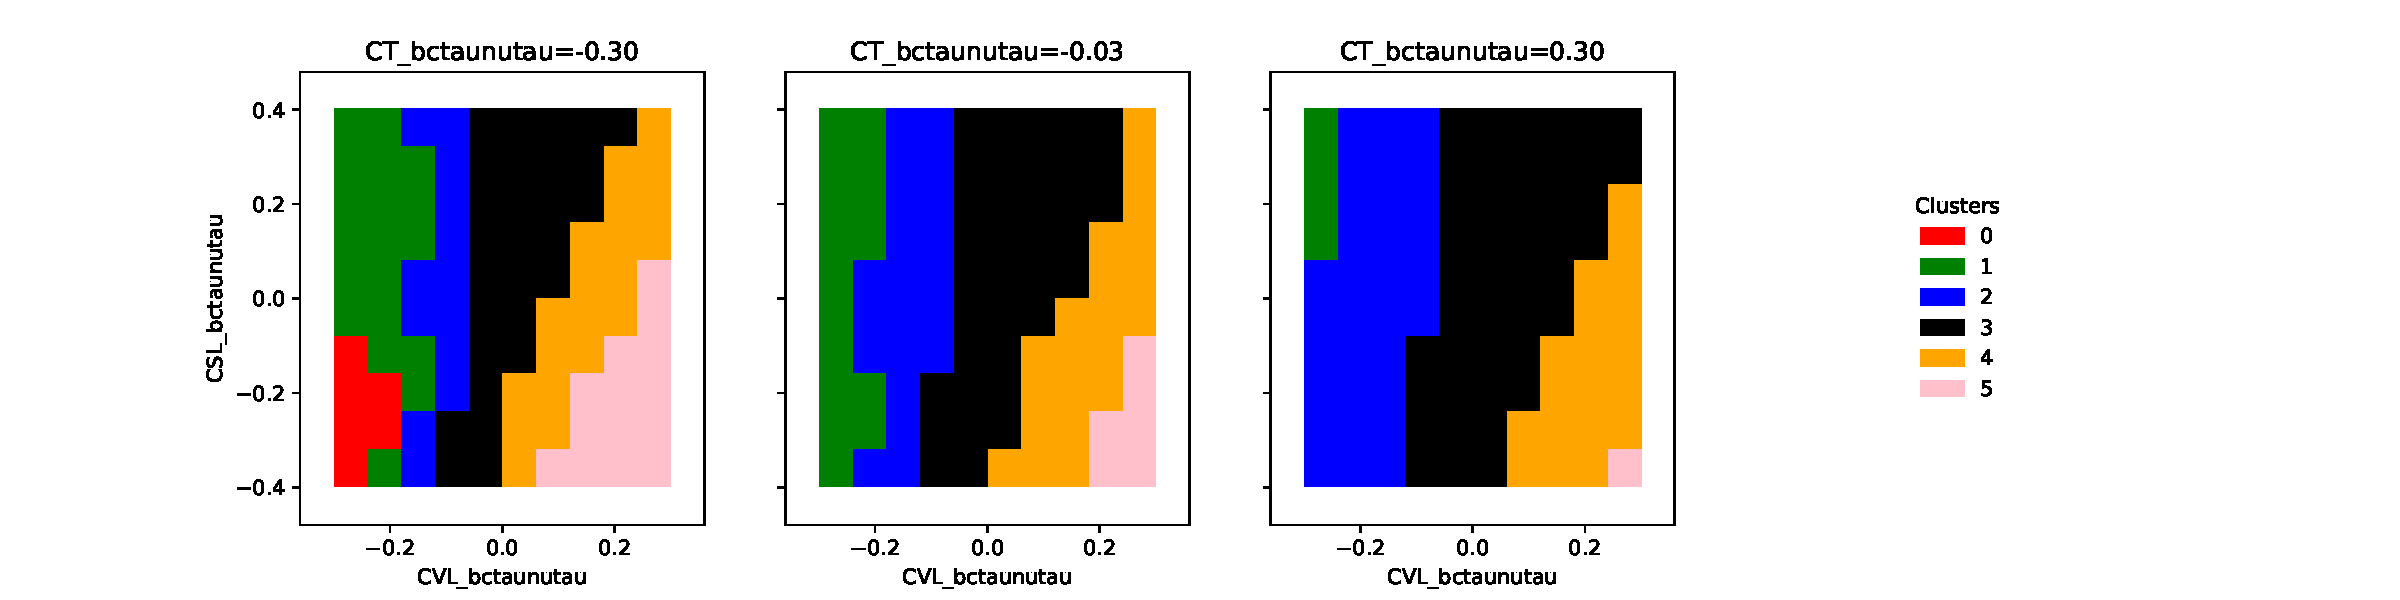
\includegraphics[trim=3cm 0 11cm 0, clip, width=10.5cm]{figures/plots/2dfill.pdf}
\end{frame}

\begin{frame}[fragile]{Software}{Quick tutorial}
    \begin{minted}[gobble=8]{python}
        d.plot_dist_box()                   # left plot
        d.plot_dist_minmax(clusters=[0,2])  # right plot
    \end{minted}
    
    \bigskip
    \begin{changemargin}{-1.2cm}{-1.2cm}
        %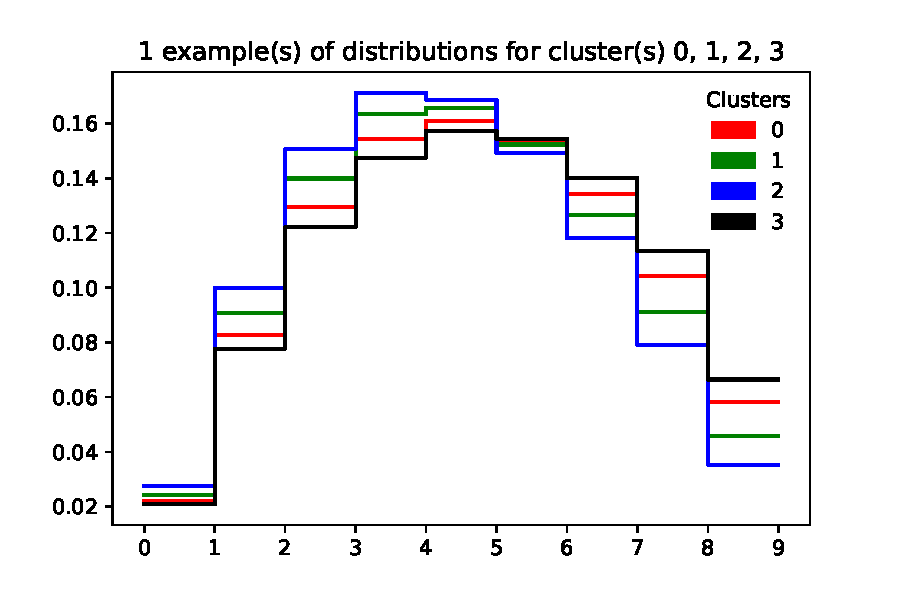
\includegraphics[width=6.8cm]{figures/plots/plot_bundles.pdf}\hspace{-0.5cm}%
        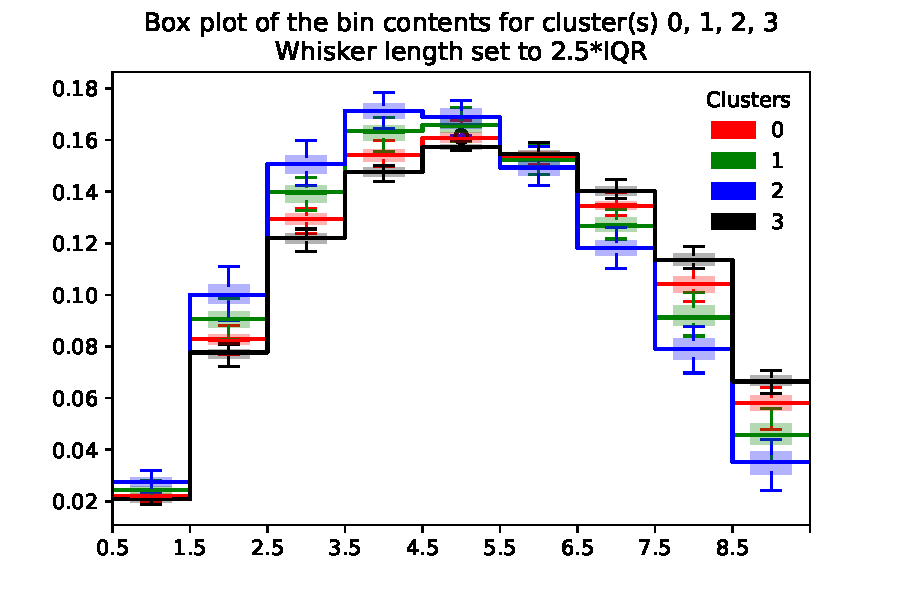
\includegraphics[width=6.8cm]{figures/plots/box_plot.pdf}\hspace{-0.5cm}
        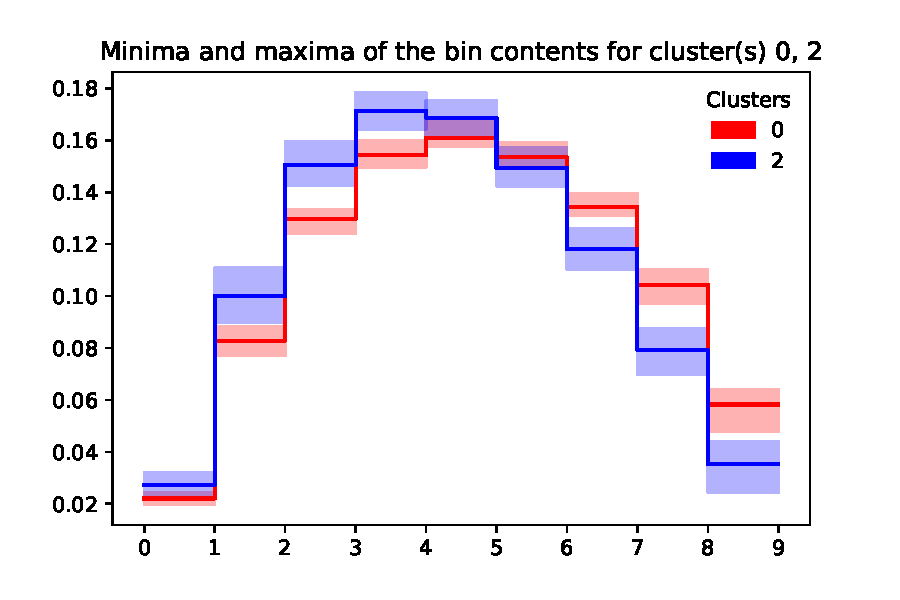
\includegraphics[width=6.8cm]{figures/plots/plot_minmax_02.pdf}\\
    \end{changemargin}
\end{frame}
\fi
